\subsection{Visão Geral}\label{4-grasews-arquitetura-visao-geral}

O desenvolvimento de Grasews segue a abordagem de desenvolvimento \textit{Domain-Driven Design} (DDD)~\cite{EVANS-2004-DDD}. 
A \figurename~\ref{fig:grasews-architectural-projects} apresenta os módulos existentes na arquitetura de Grasews distribuídos nas camadas da abordagem DDD.

\begin{figure}[h]
    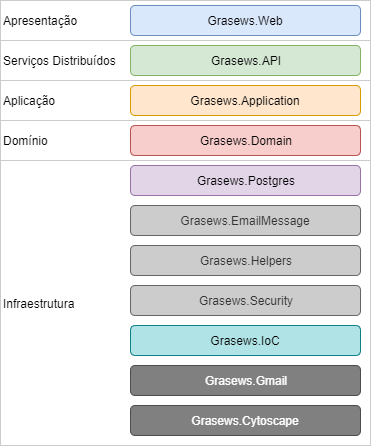
\includegraphics[scale=0.7]{4-grasews/imagens/grasews-architectural-projects.png}
    \centering
    \caption[Camadas e módulos da arquitetura da ferramenta Grasews]{\textbf{Camadas e módulos da arquitetura da ferramenta Grasews.}}
    \label{fig:grasews-architectural-projects}
\end{figure}

\newpage

A partir da abordagem DDD, a solução implementada consiste de cinco (5) camadas:

\begin{enumerate}

  \item
  \textit{\textbf{Apresentação}}:
  
  Esta camada de \textit{front-end} é composta pelo módulo \texttt{Grasews.Web}, que provê a interface gráfica de usuário (UI) da ferramenta.
  
  \item
  \textit{\textbf{Serviços Distribuídos}}:
  
  Esta camada é composta pelo módulo \texttt{Grasews.API}, que provê uma API para expor as funcionalidades do \textit{back-end} de Grasews. Esta API consiste de um conjunto de operações disponibilizadas por meio de serviços web RESTful. Todas as ações executadas por um usuário que necessitam interação com os demais módulos do lado servidor (\textit{back-end}) da aplicação são exclusivamente realizadas através da API.
  
  \item
  \textit{\textbf{Aplicação}}:
  
  Esta camada de \textit{back-end} é composta pelo módulo \texttt{Grasews.Application}, responsável por orquestrar as regras de negócio da aplicação.
  
  \item
  \textit{\textbf{Domínio}}:
  
  Esta camada de \textit{back-end} é composta pelo módulo \texttt{Grasews.Domain}, responsável por definir as regras de negócio da aplicação e as entidades de domínio do negócio. As regras de negócio são providas por meio de interfaces de desenvolvimento contidas neste módulo. Os demais módulos da aplicação seguem regras ditadas pelo módulo \texttt{Grasews.Domain}. A arquitetura de Grasews possui o seu desenvolvimento orientado a interfaces e não a implementações de classes. Tal característica facilita a substituição de um módulo da aplicação por outro módulo que, por exemplo, utiliza outra tecnologia diferente. Por exemplo, caso optemos por não usar mais o SGBD \textit{Postgres}, substituindo-o pelo SGBD \textit{Microsoft SQL Server}\cite{SQLSERVER-2019}, basta substituirmos o módulo \texttt{Grasews.Postgres} por, por exemplo, o módulo \texttt{Grasews.SqlServer}, o qual utilizaria as bibliotecas apropriadas para o acesso ao novo banco de dados. Adicionalmente, por meio das interfaces de  \texttt{Grasews.Domain}, garantimos que toda a aplicação funcione seguindo regras definidas pelo domínio (núcleo da aplicação).
  
  \item
  \textit{\textbf{Infraestrutura}}:
  
  Esta camada de \textit{back-end} é subdivida em três subcamadas de módulos: i) acesso a dados; ii) corte transversal; e iii) serviços externos.  A subcamada de acesso a dados é composta pelo módulo \texttt{Grasews.Postgres}, responsável por conectar a aplicação ao SGBD Postgres~\cite{POSTGRES-2019}. A subcamada de corte transversal é composta pelos módulos \texttt{Grasews.EmailMessage}, \texttt{Grasews.Helpers}, \texttt{Grasews.Security} e \texttt{Grasews.IoC}. O módulo \texttt{Grasews.EmailMessage} provê suporte à construção de mensagens de \textit{e-mail}. O módulo \texttt{Grasews.Helpers} provê suporte funcional às demais camadas e, consequentemente, aos demais módulos. Por exemplo, funcionalidades de suporte à leitura de XML, funcionalidades de suporte à manipulação de enumeradores e funcionalidades de suporte à requisições HTTP entre o \textit{front-end} e a API. O módulo \texttt{Grasews.Security} provê suporte à funcionalidades de segurança da aplicação. Por exemplo, funcionalidades de suporte à autenticação e permissões de um usuário. Finalmente, o módulo \texttt{Grasews.IoC} provê suporte funcional à inversão de controle (\textit{inversion of control} - IoC) e à injeção de dependências (\textit{dependency injection} - DI).
  
  A inversão de controle é uma técnica utilizada para reduzir o acoplamento entre objetos (classes) de uma arquitetura de \textit{software}. A arquitetura de um projeto pode ser severamente prejudicada quando tem-se um alto acoplamento, podendo tornar a sua manutenção custosa e até mesmo dificultar a sua evolução.
  
  A injeção de dependências é uma forma de se aplicar a inversão de controle, garantindo então um baixo acoplamento em um conjunto de classes. O padrão de injeção de dependência é baseado em abstrações das classes, por meio de classes abstratas ou interfaces de desenvolvimento. Segundo este padrão, o desenvolvimento é orientado à interface de uma classe ao invés de sua verdadeira implementação. A injeção de dependências de Grasews é feita por meio da injeção de objetos (dependências) por meio de construtores. Com isso, uma classe que necessita de instâncias de outras classes (dependências) obtém tais instâncias por meio da injeção destes objetos no construtor desta classe dependente.
  
  Por fim, a camada de serviços externos é composta pelos módulos \texttt{Grasews.Cytoscape} e \texttt{Grasews.Gmail}. O módulo de serviço externo \texttt{Grasews.Cytoscape} provê suporte à construção dos grafos WSDL e OWL da ferramenta. Este módulo utiliza a biblioteca \textit{Cytoscape.js}~\cite{CYTOSCAPE-2015}. Já o módulo de serviço externo \texttt{Grasews.Gmail} provê suporte ao envio de mensagens de \textit{e-mail} aos usuários por meio do serviço do \textit{Gmail}~\cite{GOOGLE-2019-GMAIL}.
  
\end{enumerate}